% -------------------------------------------------------------------
{
\begin{figure*}[hbt]
% \newcommand{\figWidth}{.45\linewidth}
% \newcommand{\clipfig}[1]{\psclip{\psframe[linecolor=white](0.,1.)(5.4,4.85)}\epsfig{#1}\endpsclip}
\psset{xunit=1.cm,yunit=1.cm,runit=1.cm}
% 
\renewcommand{\figWidth}{6.cm}
\newcommand{\clipfig}[2]{\clipFig{#1}{#2}{.0}{1.}{0.}{1.}}
% 
\begin{center}
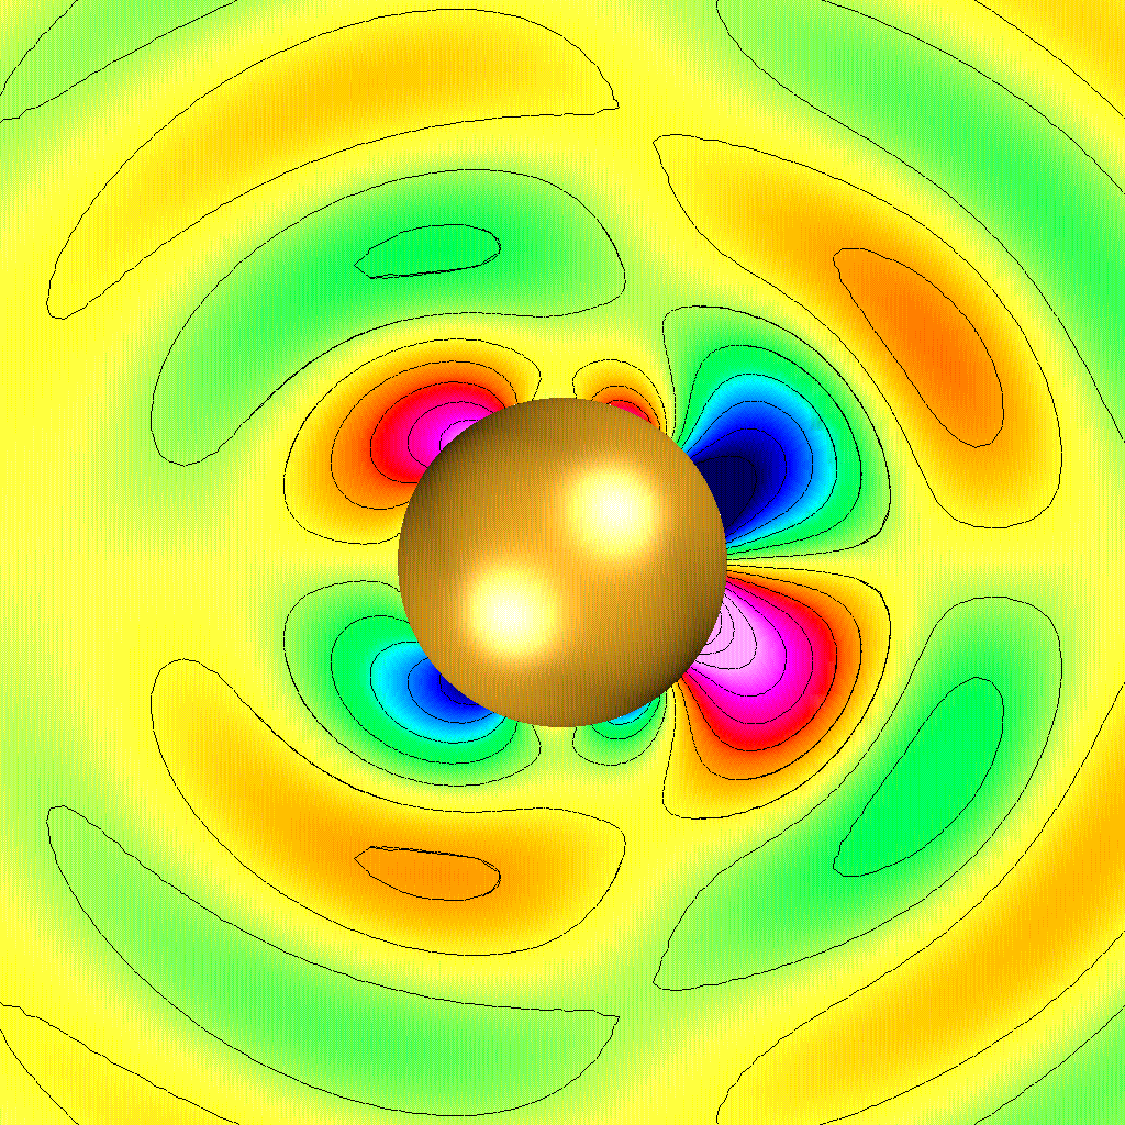
\includegraphics[width=\figWidth]{figures/scatSibx2-Ex}
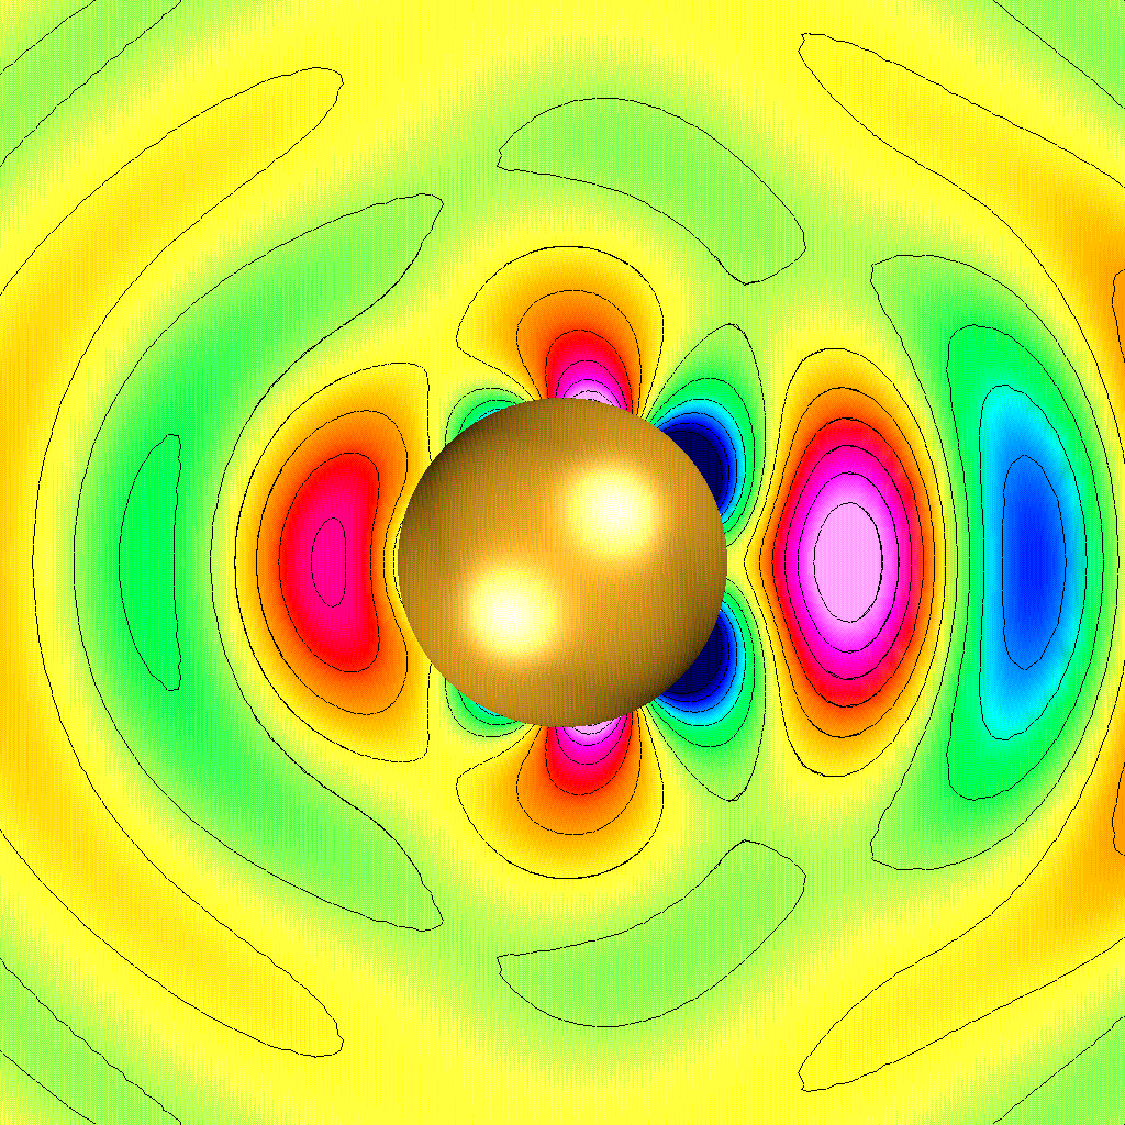
\includegraphics[width=\figWidth]{figures/scatSibx2-Ey}
%- \begin{pspicture}(0,0)(13.,6.5)
%- % \rput( 3.2,3.){\clipfig{\maxDir/scatSibx2-Ex.ps}{\figWidth}}
%- % \rput( 9.5,3.){\clipfig{\maxDir/scatSibx2-Ey.ps}{\figWidth}}
%- \rput( 3.2,3.){\clipfig{figures/scatSibx2-Ex}{\figWidth}}
%- \rput( 9.5,3.){\clipfig{figures/scatSibx2-Ey}{\figWidth}}
%- % 
%- % \rput[l](.70,11.5){\psframebox*[fillstyle=solid,fillcolor=mediumgoldenrod]{$E_X$}}
%- % \rput[l](7.0,11.5){\psframebox*[fillstyle=solid,fillcolor=mediumgoldenrod]{$E_y$}}
%- \rput[l](.70,5.5){\psframebox*[fillstyle=solid,fillcolor=mediumgoldenrod]{$E_x$}}
%- \rput[l](7.0,5.5){\psframebox*[fillstyle=solid,fillcolor=mediumgoldenrod]{$E_y$}}
%- % 
%- % \psline[linewidth=1.pt]{->}(7,-.8)(7.5,.9)
%- % turn on the grid for placement
%- % \psgrid[subgriddiv=2]
%- %
%- \end{pspicture}
\end{center}
\caption{Scattering of a plane wave by a perfectly conducting sphere. 
The scattered fields for $E_x$ and $E_y$ are shown.}
\label{fig:scatSphereFig}
\end{figure*}
}
